%!TEX root = ../thesis.tex

\thispagestyle{myheadings}

\graphicspath{{Body/Figures/ExperimentalOverview/Ring/}{Body/Figures/TrackingFigures/TrackerPics/}{Body/Figures/ExperimentalOverview/Auxiliary/}}

\chapter{Detector Systems}
\label{sec:DetectorSystems}

While the calorimeters are the primary detector and gather the most data to measure the \wa signal, there are a number of different auxiliary systems for monitoring injection and beam dynamics. These include the T0, IBMS, and fiber harps. The straw tracking detectors measure beam dynamics, but also serve as a cross check for some parameters of the calorimeter, and are used to look for a possible EDM signal. (Haven't mentioned EDMs at all at this point so maybe leave this last bit out.) Each of these systems will be described in the following sections.


\section{Auxiliary Detectors}

\subsection{T0}
\label{sec:T0}

During data taking, a reference time must be chosen so as to align all different detector systems in time. When taking data from fill to fill, decay positron spectra must be aligned in phase. Without this functionality, analyzing the data from different systems and comparing them would be impossible. To do this a ``T0'' counter is placed just on the outside of the ring before the inflector. It is made up of a scintillating paddle connected to two photo-multiplier tubes (PMTs) \cite{t0Hannah,t0Aaron}. See \figref{fig:T0counter}. One PMT, PMT A, has a 1\% neutral density filter resulting in low photo-electron stats, and acts primarily as a timing measurement. The other, PMT B, has a 10\% neutral density filter resulting in higher stats, and acts as a shape counter and proxy for fill intensity. (In general the signals are very similar.) Together they provide a measure of the injected beam profile in time, allowing to align the detectors each fill, and the data from fill to fill. Some measured T0 pulses are shown in \figref{fig:T0pulses}. The shape of the incoming pulses has a somewhat trident-like shape, with a very large spike in the middle of the time width, and two spikes on the outside edges. This shape owes itself to the accelerator complex, and varies from bunch to bunch.


\begin{figure}[]
\centering
    \begin{subfigure}[t]{0.45\textwidth}
        \centering
        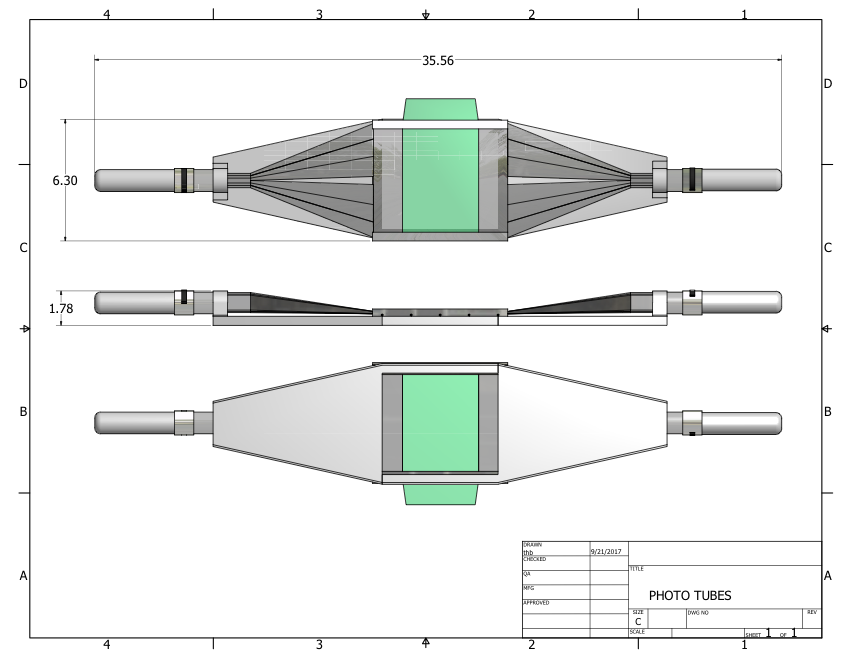
\includegraphics[width=\textwidth]{T0}
        \caption{The T0 counter is made up of a scintillator in the middle shown in green, which connects with light guides to PMTs on the left and right.}
    \label{fig:T0counter}
    \end{subfigure}%
    \hspace{1cm}
    \begin{subfigure}[t]{0.45\textwidth}
        \centering
        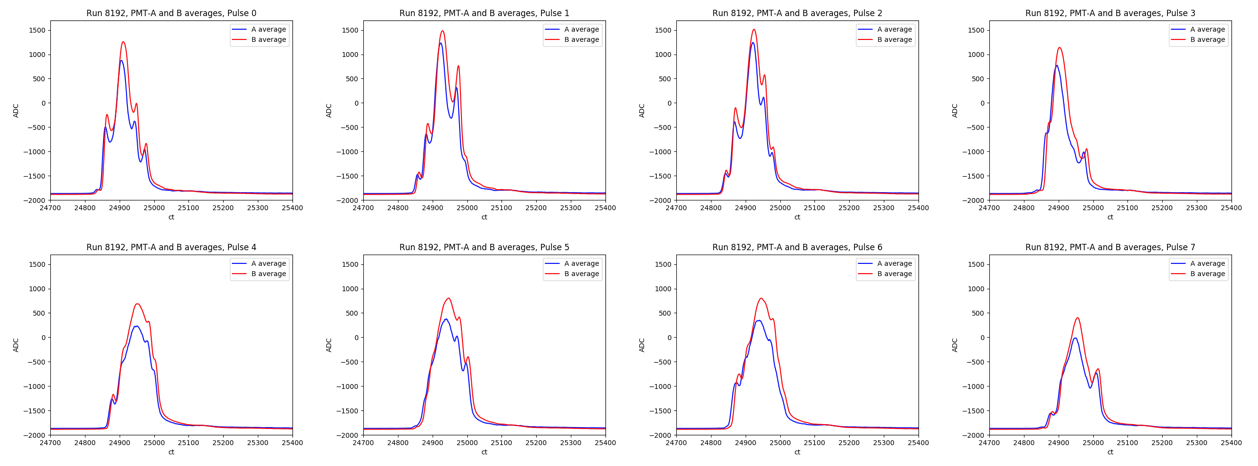
\includegraphics[width=\textwidth]{T0pulses}
        \caption{Time profiles for the two PMTs in the T0 counter for one of the eight bunches we receive at a time as described in \secref{sec:Accelerator}. Each profile is an average of 100 such profiles. The x axis is in clock ticks, each of which is $\SI{1.25}{ns}$.}
    \label{fig:T0pulses}    
    \end{subfigure}
\caption[T0 counter and pulses]{Figures from \refref{t0Hannah}.}
\label{fig:T0}
\end{figure}


\subsection{Inflector Beam Monitoring System}
\label{sec:IBMS}

While the T0 provides timing and intensity measurements, the inflector beam monitoring system (IBMS) provides measurements of the beam position properties as it passes through the inflector. This is useful because the injection aperture is so tight, and incoming beam parameters are tightly constrained. The IBMS system serves to provide a direct diagnostic handle on the phase space matching between the last accelerator components and the \gmtwo storage ring \cite{ibms1}. The IBMS is made up of two scintillating fiber detectors, as shown in \figref{fig:IBMS1and2}. These devices are placed at the outside of the magnet yoke before injection into the back hole of the magnet, and at the entrance to the inflector \cite{ibms2}. A third device is planned to be at or near the downstream end of the inflector. See \figref{fig:IBMSPlacement}. 


\begin{figure}[]
    \centering
    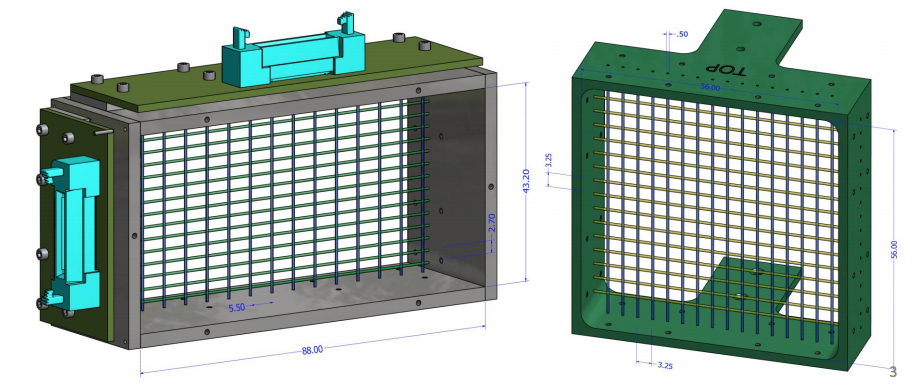
\includegraphics[width=0.9\textwidth]{IBMS1and2}
    \caption[IBMS Models]{Simulation models of the IBMS 1 and 2 detectors. Scintillating fibers form an array which detect particles as they pass through them.}   
    \label{fig:IBMS1and2}
\end{figure}

\begin{figure}[]
    \centering
    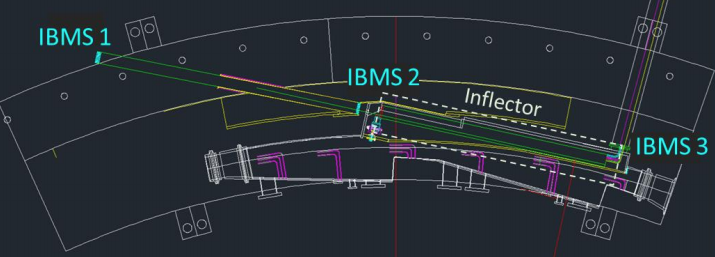
\includegraphics[width=0.9\textwidth]{IBMSPlacement}
    \caption[IBMS Positions]{The positions of IBMS 1, 2, and the planned 3rd device are shown with respect to the vacuum chamber and inflector.}   
    \label{fig:IBMSPlacement}
\end{figure}



\subsection{Fiber Harps}
\label{sec:FiberHarps}

The last auxiliary detector is the so called ``fiber harp'' system. It is made up of four scintillating fiber detectors located within the ring that serve to measure the beam intensity as a function of time and position \cite{fiberharp}. Two of the detectors measure the radial components of the beam, and two measure the horizontal components. The fiber harps are located at points 180\textdegree{} and 270\textdegree{} from the inflector. One of these devices is shown in \figref{fig:fiberharp}. The fiber harps have the added advantage that they are able to measure beam properties throughout the fill, providing a diagnostic tool which is sensitive to the scraping procedure and the CBO properties of the beam. An example of fiber harp measurements is shown in \figref{fig:fiberharp_measurement}. However because the fiber harps are a destructive measurement of the beam due to multiple scattering in the fibers, the system was designed to be retractable. They are inserted during special diagnostic or systematic runs, and are pulled out of the beam path during production data taking.


\begin{figure}[]
\centering
    \begin{subfigure}[t]{0.45\textwidth}
        \centering
        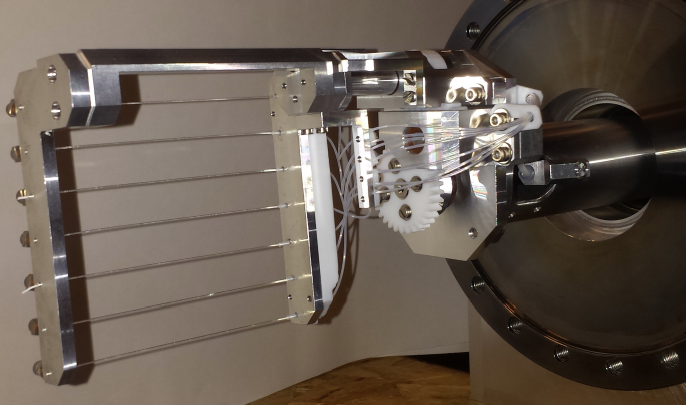
\includegraphics[width=\textwidth]{fiberharp}
        \caption{Picture of one of the fiber harps. A row of seven scintillating fibers measures the beam intensity as a function of time at vertical or horizontal positions depending on which fiber harp is inserted.}
    \label{fig:fiberharp}
    \end{subfigure}%
    \hspace{1cm}
    \begin{subfigure}[t]{0.45\textwidth}
        \centering
        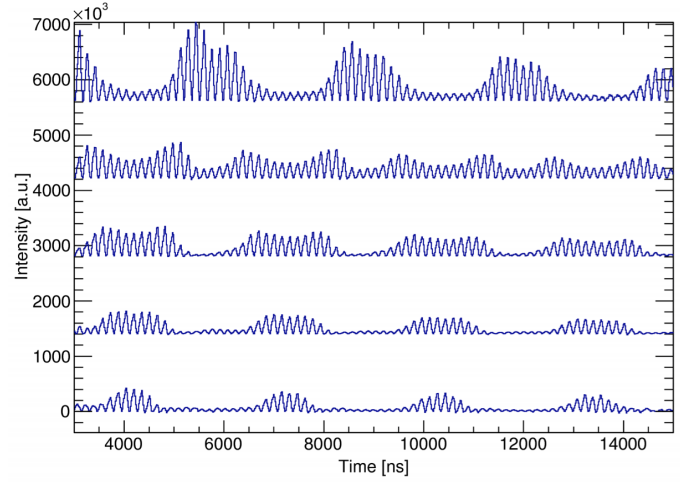
\includegraphics[width=\textwidth]{fiberharp_measurement}
        \caption{Shown are fiber harp beam intensity measurements for the horizontal fiber harp. Each spectra is from a single fiber, with the spectra at the top being at the greatest radial positions. The fast oscillations of the cyclotron frequency can be seen along with the slower oscillations of the CBO.}
    \label{fig:fiberharp_measurement}
    \end{subfigure}
\caption[Fiber harp and measurement]{F}
\label{fig:fiberharp_measurement}
\end{figure}






\section{Calorimeters}
\label{sec:Calorimeters}

% what they do
% what they are
% how they work

Electromagnetic calorimeters measure the times and energies of decay positrons as they curl inward from the storage region. There are 24 calorimeters located symmetrically around the inside of the ring in close proximity to the vacuum chamber, as shown in \figref{fig:TrackerCaloWithLines}. They lie close to the storage region in order to measure a large fraction of the total number of observable decay positrons, including the high energy decay positrons which curl inward only slightly more than the muons themselves do. (max acceptance)

Each calorimeter consists of 54 channels of PbF\textsubscript{2} crystals arrayed in a 6 high by 9 wide array, which measure Cerenkov light emitted by the incident positrons as they pass through the crystals \cite{Fienberg:2014kka}. (Picture of single calo and its crystals here.) Cerenkov light is naturally fast which improves timing resolution of the incoming hits. Each crystal is 2.5 x 2.5 x 14 cm\textsuperscript{3} and is wrapped in black Tedlar\textregistered\ foil to reduce light transmission between crystals and improve position reconstruction, as well as reduce pulse width \cite{Kaspar:2016ofv}. The light is read out by large area silicon photo-multiplier (SiPM) sensors. Each calorimeter sits on a board extending out from a cart containing the electronic which power the calorimeters and read out the data, as shown in Figure \ref{fig:} This is to relocate magnetic material away from the field region to avoid perturbing the field and to remove sensitive electronics from the decay path region. Similarly, due to the close proximity to the storage region and by extension the magnetic field, the calorimeters, the encapsulating material, and the SiPMs are made from non-magnetic material.

In order to determine \amu to the precision goal, there are modest requirements on the performance of the calorimeters. They must have a relative energy resolution of better than 5\% at 2 \GeV, in order for proper event selection \cite{TDR}. They must have a timing resolution of better than 100 ps for positrons with greater than 100 \MeV energy. The calorimeters must be able to resolve multiple incoming hits through temporal or spatial separation at 100\% efficiency for time separations of greater than 5 ns in order to reduce the pileup systematic error due to the high rate. Finally, the gain of the measured hits must be stable to $<$ 0.1\% over a 200 $\mu$s time period within a fill, and unaffected by a pulse arriving in the same channel a few nanoseconds earlier. The long term gain stability over a time period of order seconds must be $<$ 1\%. The SiPMs chosen satisfy these requirements (as well as the physical ones), due to their fast rise times and consistent pulse shapes. (Should this part be here? Or elsewhere? Before perhaps? Might need to update the gain numbers...)

(I've condensed quite a bit this section from the TDR - is that okay?)

A 12 bit waveform digitizer (WFD) samples each photodetector channel at a rate of 800 MSPS with a 1 Gb memory buffer and the data are transferred to a bank of GPU processors for on-line data processing \cite{Sweigart:2016jty}. The timing resolution of these WFDs is $<$ 50 ps for most pulse amplitudes.

Should I go into the calorimeter DAQ here? Or make that it's own section - how uniform are the DAQ systems for each detector system? Are the same sorts of modules and crates and WFDs used or what? If so it's own section might make sense, otherwise probably include small pieces at the end of each individual detector about the daq system

\begin{figure}[]
    \centering
    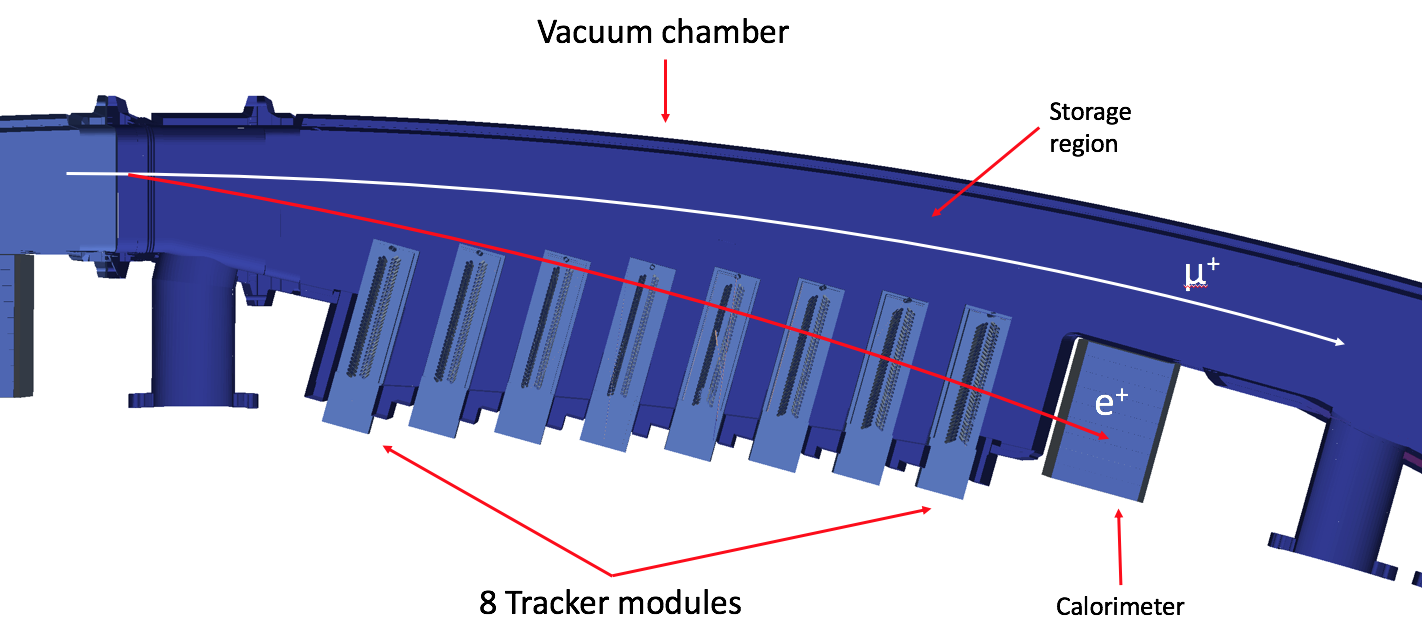
\includegraphics[width=0.9\textwidth]{TrackerCaloWithLines}
    \caption[TrackerCaloWithLines]{Birds eye view of a model of a vacuum chamber containing a tracker station, and the associated calorimeter. Muons pass around the ring in the center of the storage region which is contained within the bulk of the vacuum chamber. The muons decay to positrons, some of which then pass through the trackers or hit calorimeters. Each tracking station consists of 8 tracker modules.}   
    \label{fig:TrackerCaloWithLines}
\end{figure}



-talk about cerenkov radiation if I haven't already
-briefly mention and explain pileup
-be sure to talk about gain as well




\subsection{Laser Calibration System}
\label{LaserCalibrationSystem}
% should I make this it's own section? or include at the end of the calo section? probably the latter

In order to satisfy the gain requirements, a laser calibration system was put into place in order to monitor the SiPM responses over short times (fill level), and long term (days to years). By comparing a known signal to the SiPM output. At the front face of each calorimeter is a board containing prisms connected to fibers from the laser system which can be pulsed in-fill or out of fill for each crystal individually. 


-can pulse laser in fill, out of fill, and double pulse
-mention the laser hut at all? probably not


% make sure these are ordered properly - might not need all of them
\cite{Anastasi:2015ssy}
\cite{Anastasi:2016luh}
\cite{Anastasi:2017sos}




\section{Straw Trackers}
\label{sec:StrawTrackers}

As described in \secref{sec:muonbeamdynamics}, the muon beam moves dynamically within the storage ring. As explained in \secref{sec:MagneticField}, the muon beam distribution ties into the measurement of the magnetic field. The primary detector system used to measure this behavior and determine the muon beam distribution is the ``straw tracker'' system. The straw trackers characterize the beam in a non-destructive fashion by measuring decay positron trajectories and extrapolating back into the storage ring. They serve to provide the direct measurement of the pitch correction as described in \secref{sub:pitch_correction}. The straw tracker measurements of beam tie directly into the calorimeter \wa analysis as will be talked about later. Decay positron trajectories can also be extrapolated forwards into the calorimeter, thus making the straw trackers a useful diagnostic tool for cross-checking calorimeter measurements, and specifically helping to resolve pileup (be sure to talk about this in the calorimeter section - since this isn't actually done yet do I even want to say this?) The details of the track reconstruction and analysis will be given in \chapref{chapter:TrackReconstruction}. Here will be given a description of the detectors themselves.





With three trackers, approximately 5\% of decaying muons will result in measurable positron tracks assuming no pileup in the tracker, many of which do not hit the nearest calorimeter.

Each tracker module consists of 4 layers of 32 straws with a stereo angle of 7.5 degrees, the first two ``U'' layers oriented with the tops of the straws at a greater radial position, and the second two ``V'' layers oriented with the bottoms of the straws at a greater radial position. A tracking module is shown in \figref{fig:tracker}. There are 2 tracker stations located in front of calorimeters 13 and 19, or at approximately 180 and 270 degrees counting clockwise from the top most point of the ring where the inflector resides. \figref{fig:WorldCoordSys} shows this. (A third station sits empty after the inflector.) Each station consists of 8 tracking modules arranged in a staircase pattern that follows the curvature of the ring as seen in \figref{fig:staircase}.

\begin{figure}[]
    \centering
    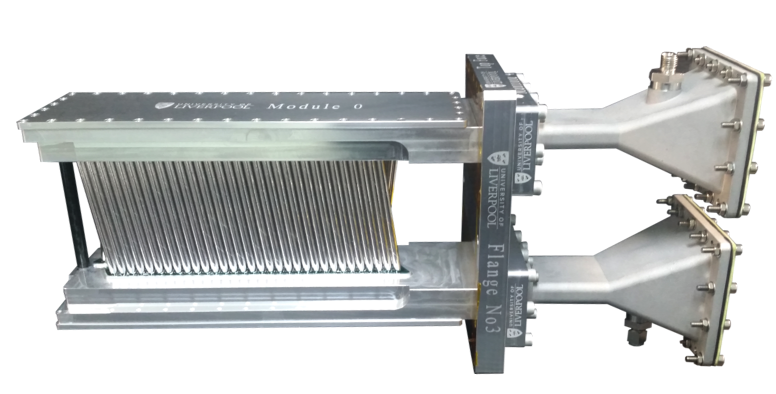
\includegraphics[width=0.9\textwidth]{Tracker}
    \caption[Tracker module]{Shown is a picture of one of the many tracking modules used in the Muon \gmtwo experiment. The first layer of straws with a stereo angle of 7.5 degrees can be seen, with the other 3 straw layers hiding behind it. The beam direction is roughly into the page in this picture, to the left of the end of the module, and this view is what the decay positrons will see.}
    \label{fig:tracker}
\end{figure}

\begin{figure}[]
    \centering
    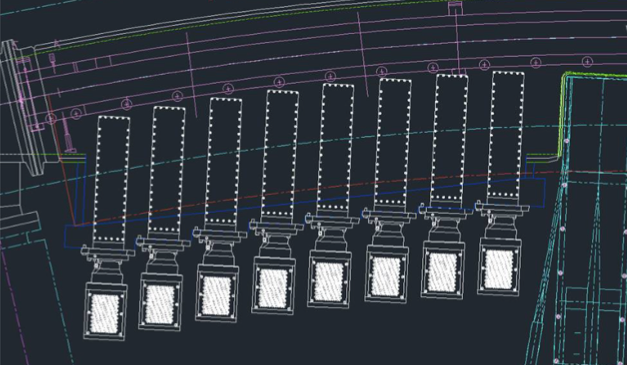
\includegraphics[width=0.9\textwidth]{trackerStation}
    \caption[Tracker module arrangement]{Tracker modules are arranged in the shown staircase pattern. In green and dark blue is the edge of the vacuum chamber (where the dark blue identifies the modification that was made to the old vacuum chambers), and it can be seen that vacuum chamber walls lie at the ends of the outside tracking modules. The position of a calorimeter can be seen in cyan at the right. The dark red spots are the locations of the outside magnet pole tips. From the shown geometry one can see that many positrons will hit either the tracker or the calorimeter but not both due to the acceptance differences.}
    \label{fig:staircase}
\end{figure}

In order to reduce the amount of multiple scattering within the straw tracking chambers as particles pass through them, the material of the straw trackers is minimized. Each straw is made of mylar foil, within which a 25 $\mu$m radius tungsten wire resides, and is filled with Argon-Ethane gas \cite{something}. Fast moving particles ionize the gas as they pass through it, and the resulting ions are drawn to the wire which is held at high voltage. When they reach the wire (and the mylar) a signal can be read out which tells us that a particle was seen to pass through the straw. By combining many such signals in a brief time span, we are able to construct tracks of incident particles. (See section blah.) The resolution of hits within the straws is approximately 150 $\mu$m \cite{something}.

The signals of the straws are read out through...







-motivation and purpose
-non-destructive measurement
-ability to measure many different things (beam, calo matching, EDM maybe)
-mention how the measurements tie into the calorimeter stuff too
-how they work
-explanation of readout electronics 
-potential some work I've done on the boards - ignore the overall construction though
-two trackers and how they should measure hits all around the ring
-reference the following chapter on the straw tracking analysis










